\documentclass{article}
\usepackage{graphicx}
\topmargin=0.0in %length of margin at the top of the page (1 inch added by default)
\oddsidemargin=0.0in %length of margin on sides for odd pages
\evensidemargin=0in %length of margin on sides for even pages
\textwidth=6.5in %How wide you want your text to be
\marginparwidth=0.5in
\headheight=0pt %1in margins at top and bottom (1 inch is added to this value by default)
\headsep=0pt %Increase to increase white space in between headers and the top of the page
\textheight=9.0in %How tall the text body is allowed to be on each page
\newcommand\tab[1][3cm]{\hspace*{#1}}
\begin{document}
	
	\begin{center}
		{
			\large\textbf{ABHISHEK ACHARYA}
		}
		
	\end{center}
	
	\begin{flushleft}
		NIT Meghalaya, 		\hspace{2.8in}    		    Contact: +91-8014692750            \\
		Bijini Complex, 		\hspace{2.85in}		    e-mailid: abhi11796acharya@gmail.com
		Laitumukhrah, \\
		Shillong-793003,     \\
		Meghalaya       \\
	\end{flushleft}
	\vspace{-0.3in}
	
	\begin{figure}[h]
		\hspace{4.4in}
		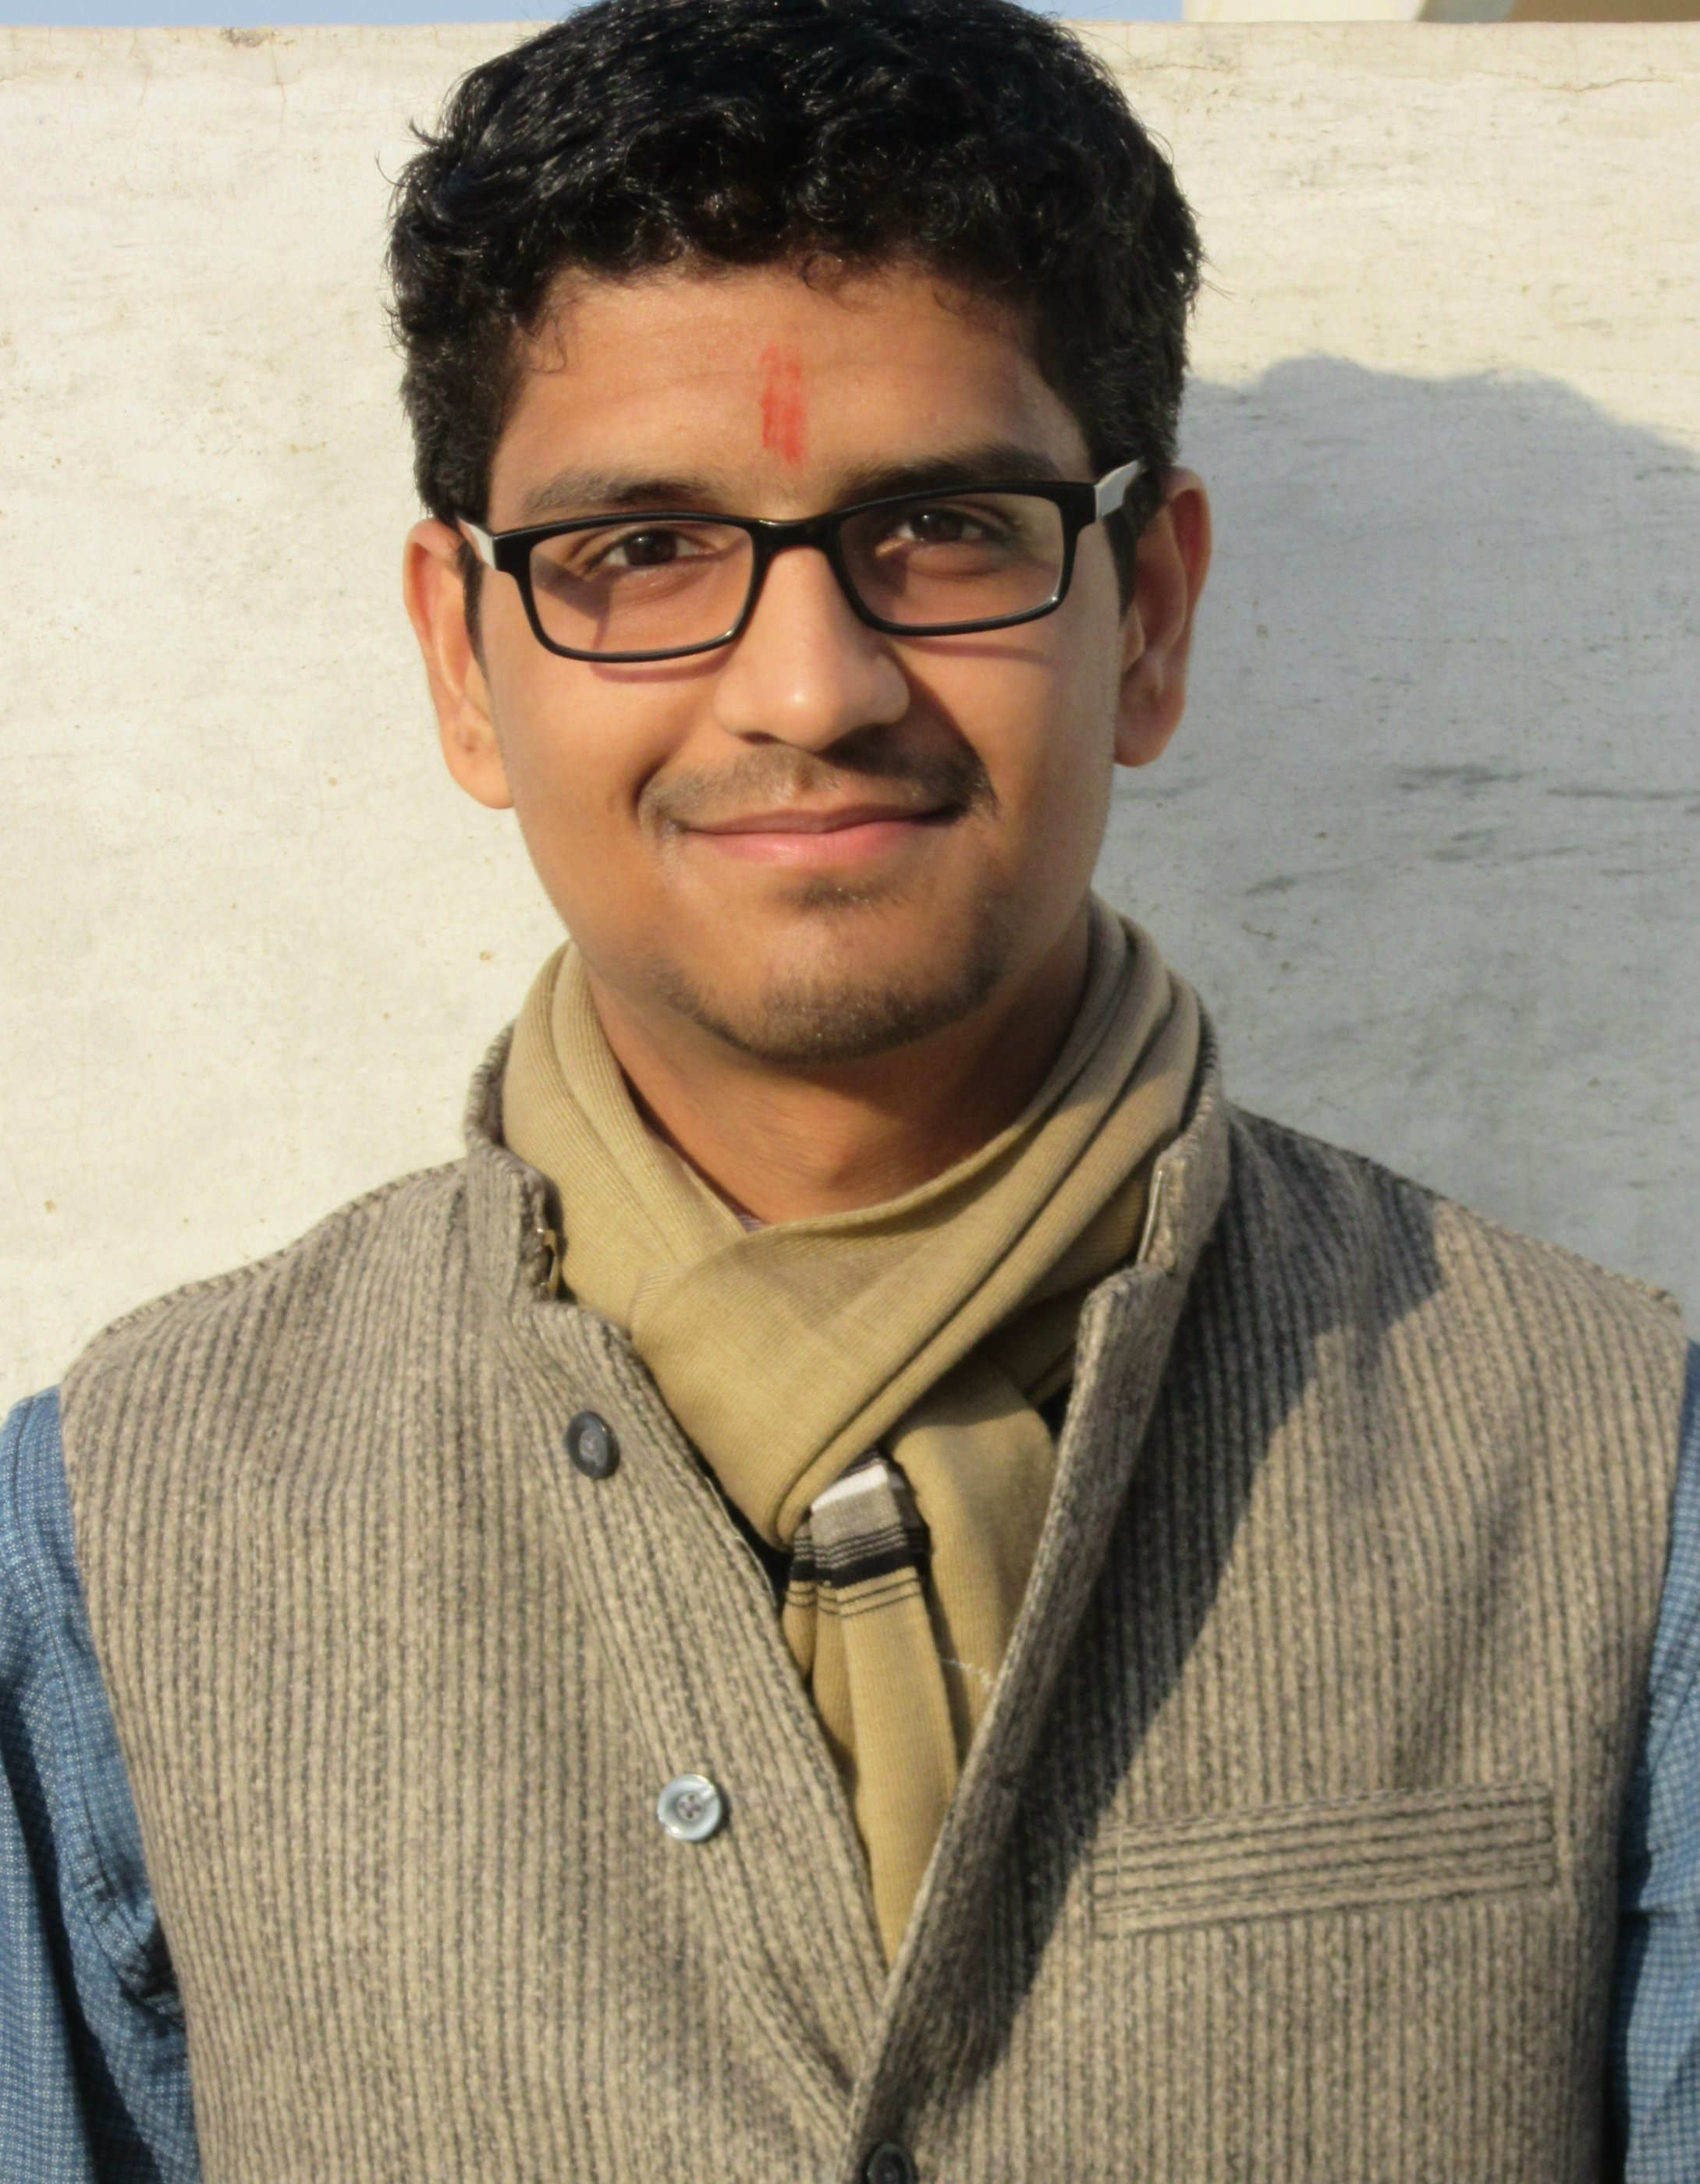
\includegraphics[width=90px]{Abhishek}
	\end{figure}
	
	%%%%%%%%%%%%%  OBJECTIVE   %%%%%%%%%%%
	\begin{flushleft}
		\textbf{OBJECTIVE}
		
		\vspace{-0.20in}
		\hspace{1.5in}
		To enhance my technical skills and implement it for mankind.\\
	\end{flushleft}
	
	%%%%%%%%%%%%   EDUCATION   %%%%%%%%%
	\begin{flushleft}
		
		\textbf{EDUCATION}
	\end{flushleft}
	
	\begin{tabular}{|c|c|c|c|c|}
		\hline
		\textbf{Certificate} & \textbf{School/College} & \textbf{Board/University} &  \textbf{year} & \textbf{Pass}   \\
		&        &            &              & \textbf{Percentage}\\
		\hline
		
		Secondary & Basic English Sr. & Board of Secondary Education & 2010-2011 &88.17 \\
		Examination&Sec. School,Bikaner & Rajasthan, Ajmer& & \\
		\hline
		Sr. Secondary & Basic English Sr. & Board of Secondary Education & 2012-2013 &82.68 \\
		Examination&Sec. School,Bikaner & Rajasthan, Ajmer& & \\
		\hline
		B.Tech & National Institute & National Institute of  & 2013-2017 &7.77 CGPA\\
		(E.E.E)	&of Technology &Technology Meghalaya, & &(Till five \\
		& Meghalaya &Shillong-793003& &Semester) \\
		\hline
	\end{tabular}
	
	 %%%%%%%%%%%%%%%   PROJECTS     %%%%%%%%%%5
	 \begin{flushleft} 
	 	\vspace{0.2in}
	 	\textbf{PROJECTS}
	 	\begin{enumerate}
	 		\vspace{-0.29in}
	 		\addtolength{\itemindent}{1.359in}
	 		\item  Working on Swarm Robotics under Creativity project Theme of Robotics and\\ \hspace*{3.5cm}IOT club, NIT Meghalaya.
	 		\item  Working on Smart Home Theme of Robotics and IOT club ,NIT Meghalaya.
	 		\item  e-Yantra Robotics research project on Hazardous Waste Disposal Theme\\ \hspace*{3.5cm}in e-yantra-2015. 
	 		\item  Wireless communication system based on ASK modulation using encoders \\\hspace*{3.5cm}and decoders.  
	 		\item  Line follower robot using ATMEGA-16 Microcontroller.
	 	\end{enumerate}
	 \end{flushleft}
	 
	 %%%%%%%%%%%%  		training and internship 	%%%%%%%%
	 \begin{flushleft} 
	 	\vspace{0.4in}
	 	\textbf{TRAINING \& \\ INTERNSHIP}
	 	\hspace{1.5cm} \textbf{NIL}
	 \end{flushleft}
	 
	  %%%%%%%%%%%%%%%%%%%%%%   Research and pub. %%%%%%%%%%
	  \begin{flushleft} 
	  	\vspace{0.4in}
	  	\textbf{RESEARCH \\ PUBLICATION}
	  	\begin{enumerate}
	  		\vspace{-0.45in}
	  		\addtolength{\itemindent}{1.359in}
	  		\item  Currently working for research paper on Slack Bus Analysis of IEEE-14 and\\\hspace{3.4cm} IEEE-30 Bus system.
	  	\end{enumerate}
	  \end{flushleft}
	  
	   %%%%%%%%%%%      technical skill %%%%%%%%	
	   \begin{flushleft}
	   	\vspace{1.15in}
	   	\textbf{TECHNICAL  \\ SKILL}
	   	\begin{itemize}
	   		\vspace{-0.45in}
	   		\addtolength{\itemindent}{1.359in}
	   		\item  Familiar in following Programming Languages 
	   		{\begin{itemize}
	   				\addtolength{\itemindent}{1.359in}
	   				\item C language
	   				\item C++ language
	   				\item assembly language
	   				\item Embedded C 	
	   			\end{itemize}
	   		}  
	   		\item Knowledge of following micro controller and micro-processor
	   		{\begin{itemize}
	   				\addtolength{\itemindent}{1.359in}
	   				\item 8051 Microcontroller 
	   				\item 8085 and 8086 Microprocessor
	   				\item ATMEGA16 Microcontroller
	   				\item ATMEGA2560 Microcontroller	
	   			\end{itemize}
	   		}  
	   		
	   		\item Familiar with following Simulation Software
	   		{\begin{itemize}
	   				\addtolength{\itemindent}{1.359in}
	   				\item Proteus 8 
	   				\item Atmel Studio
	   				\item Keil uVision
	   				\item Power System Simulator for Engineers (PSS@E)
	   				\item Matlab/Simulink 
	   				\item Orcad Pspice 	
	   			\end{itemize}
	   		} 
	   	\end{itemize}
	   \end{flushleft}
	   
	     	 	%%%%%%%%%%		soft skill		%%%%%%%%
	     	 	\begin{flushleft} 
	     	 		
	     	 		\vspace{0.4in}
	     	 		\textbf{SOFT SKILL}
	     	 		\begin{enumerate}
	     	 			\vspace{-0.30in}
	     	 			\addtolength{\itemindent}{1.359in}
	     	 			\item Leadership
	     	 			\item Communication  
	     	 			\item Management 
	     	 		\end{enumerate}
	     	 	\end{flushleft}
	     	 	
	     
	\end{document}